\documentclass[10pt,compress,serif,aspectratio=169]{beamer}
\usepackage{pres2023_169}
\usepackage[utf8]{inputenc}
\graphicspath{{figures/}}
 
%\author[JTCAM]{G. Anciaux}
%
%\title[JTCAM]{Why not \textit{Diamond Open Access} ?}
\begin{document}

\begin{frame}[t]
  \begin{center}
  \vspace{1cm}
  {\huge Why not \textit{Diamond Open Access} ?}\\
  \vspace{.5cm}
  {\Large Guillaume Anciaux}\\{LSMS, IIC, ENAC, EPFL}\\
  \end{center}
  \vspace{1cm}
  \fig{.45}{OA_acc_to_phd_comics}
  \begin{center}
    \small
    Graphic from \href{http://www.phdcomics.com/comics.php?f=1533}{PHD Comics}
  \end{center}
\end{frame}


%\usebackgroundtemplate{
\includegraphics[width=12.8cm,height=9.6cm]{cover2.pdf}}{\begin{frame}[t,plain]\end{frame}}
%\usebackgroundtemplate{
\includegraphics[height=10cm]{bg.pdf}}

%%%

\begin{frame}[t]{Introduction}

\end{frame}
%%%

\begin{frame}[t]{Outlook}
\begin{columns}[t]
        \begin{column}{.5\textwidth}
            \tableofcontents[sections={1-3}]
        \end{column}
        \begin{column}{.5\textwidth}
            \tableofcontents[sections={4-6}]
        \end{column}
    \end{columns}
\end{frame}

\section{History of (academic) press}
\begin{frame}[t]{A small history of (Academic) Press...}

  References:\\

  \begin{itemize}
    \item 
  \href{https://www.theguardian.com/science/2017/jun/27/profitable-business-scientific-publishing-bad-for-science}{S. Buranyi, Is the staggeringly profitable business of scientific publishing bad for science? The Guardian (2017)}.
  \item
    \href{https://doi.org/10.5281/zenodo.7212922}{Against Parasite Publishers: Making Journals Free (2022)}
\end{itemize}
    \vfill
\pause
  \begin{center}
    That are \alert{\Large highly} recommended to read...
  \end{center}
\vfill
  \fig{.5}{Open_Access_Explained}
  \begin{center}
    \small
    Graphic from \href{http://www.phdcomics.com/comics.php?f=1533}{PHD Comics}
  \end{center}
\end{frame}
\subsection{Foundation}
\begin{frame}[t]%
 \titleframe{History}\vskip1cm%

{\large First scientific press:\newline}
 
 \begin{itemize}


 \item 1450: Printing Press (in europe)
 \item 1534: Foundation of Cambridge University Press
   %Foundation of Cambridge University Press, the oldest university press and publishing house in the world
 \item 1665: \textit{Journal des Sçavans} (France), \textit{Philosophical Transactions of the Royal Society} (UK)\\
   %Creation of Le Journal des Sçavans in France, the first academic journal. Soon after, the Philosophical Transactions of the Royal Society appears in the UK. It still exists today[5]. The familiar functions of the scientific journal –registration, certification, dissemination, and archiving– are already present[6]
 \end{itemize}

 \vfill
 \pause
{\large Defined the purpose of scientific journals:\newline}

\begin{itemize}
\item registration: authorship/priority claim
\item certification: usually peer-review
\item dissemination: provide (targeted) access
\item archiving: permanent access link (citable) 
\end{itemize}
\end{frame}

 %%%
\subsection{Authors rights}

\begin{frame}[t]%
 \titleframe{Author and Copy rights}\vskip1cm%
\begin{itemize}

 \item 1710: \textit{Statute of Anne}: British authors can control the copying of their books 
   % Royal assent to the Statute of Anne. The British authors are granted the right to control the copying of their books. The duration of copyright is 14 years(renewable once), after which the books enter the public domain[7]. This new regime follows a period of censorship and monopoly(by the Stationer’s Company) and a period of no regulation, which called for a new licensing protecting the authors
 \item 1852: articles published (in FR/UK) can be freely reprinted and translated (unless reserved rights are explicitly mentioned)
   % Signature of a bilateral treaty between the UK and France: all articles published abroad in periodicals can be freely reprinted and translated, unless reserved rights are explicitly mentioned[8]
 \item Foundation of Nature (1869) and Elsevier (1880)
   %Foundation of the British scientific journal Nature[9]
 %1880: Foundation of the Dutch publishing company Elsevier[10]
 \item 1886: Berne Convention governing copyright: grants a CC BY licence by default.%Signature of the Berne Convention, an international agreement governing copyright. Its article 7 states: “Articles from newspapers or periodicals published in any of the countries of the Union may be reproduced in original or in translation in other countries of the Union, unless the authors or publishers have expressly forbidden it.” [11] In today’s parlance, the Berne Convention grants a CC BY licence by default.

 \item 1908: Berlin Act reverses the standards: reproduction implicitly forbidden. %1908: Berlin Act: revision of the Berne Convention. It reverses the standards: instead of being implicitly allowed, reproduction is now implicitly forbidden. Its article 9 states: “Serial stories, tales, and all other works, whether literary, scientific, or artistic, whatever their object, published in the newspapers or periodicals of one of the countries of the Union, may not be reproduced in the other countries without the consent of the authors.” The Berne convention has later been further updated, but this restriction remains. Most countries have now signed it [11].
 \item 1928: Rome Act: author’s rights $\neq$ copyright
   %1928: Rome Act: revision of the Berne Convention. The article 6bis states: “Independently of the author’s copyright, and even after transfer of the said copyright, the author shall have the right to claim authorship of the work, as well as the right to object to any distortion, mutilation or other modification of the said work which would be prejudicial to his honour or reputation.”. This implements the moral rights of the authors, which is an essential feature of the author’s rights or droit d’auteur, as opposed to the copyright.
 \end{itemize}
\end{frame}

 %%%

\subsection{Research Budgets}

\begin{frame}[t]{History}
{
 \begin{center}
   \Large Post-World War II\\ Research budgets increase enormously
 \end{center}
}
 \begin{quote}The average yearly growth of the US federal budget dedicated to non-defense R\&D between 1953 and 1973 is more than 15\%
 \end{quote}
\end{frame}

\begin{frame}[t]{US Budgets}
\only<1>{
 \begin{center}
 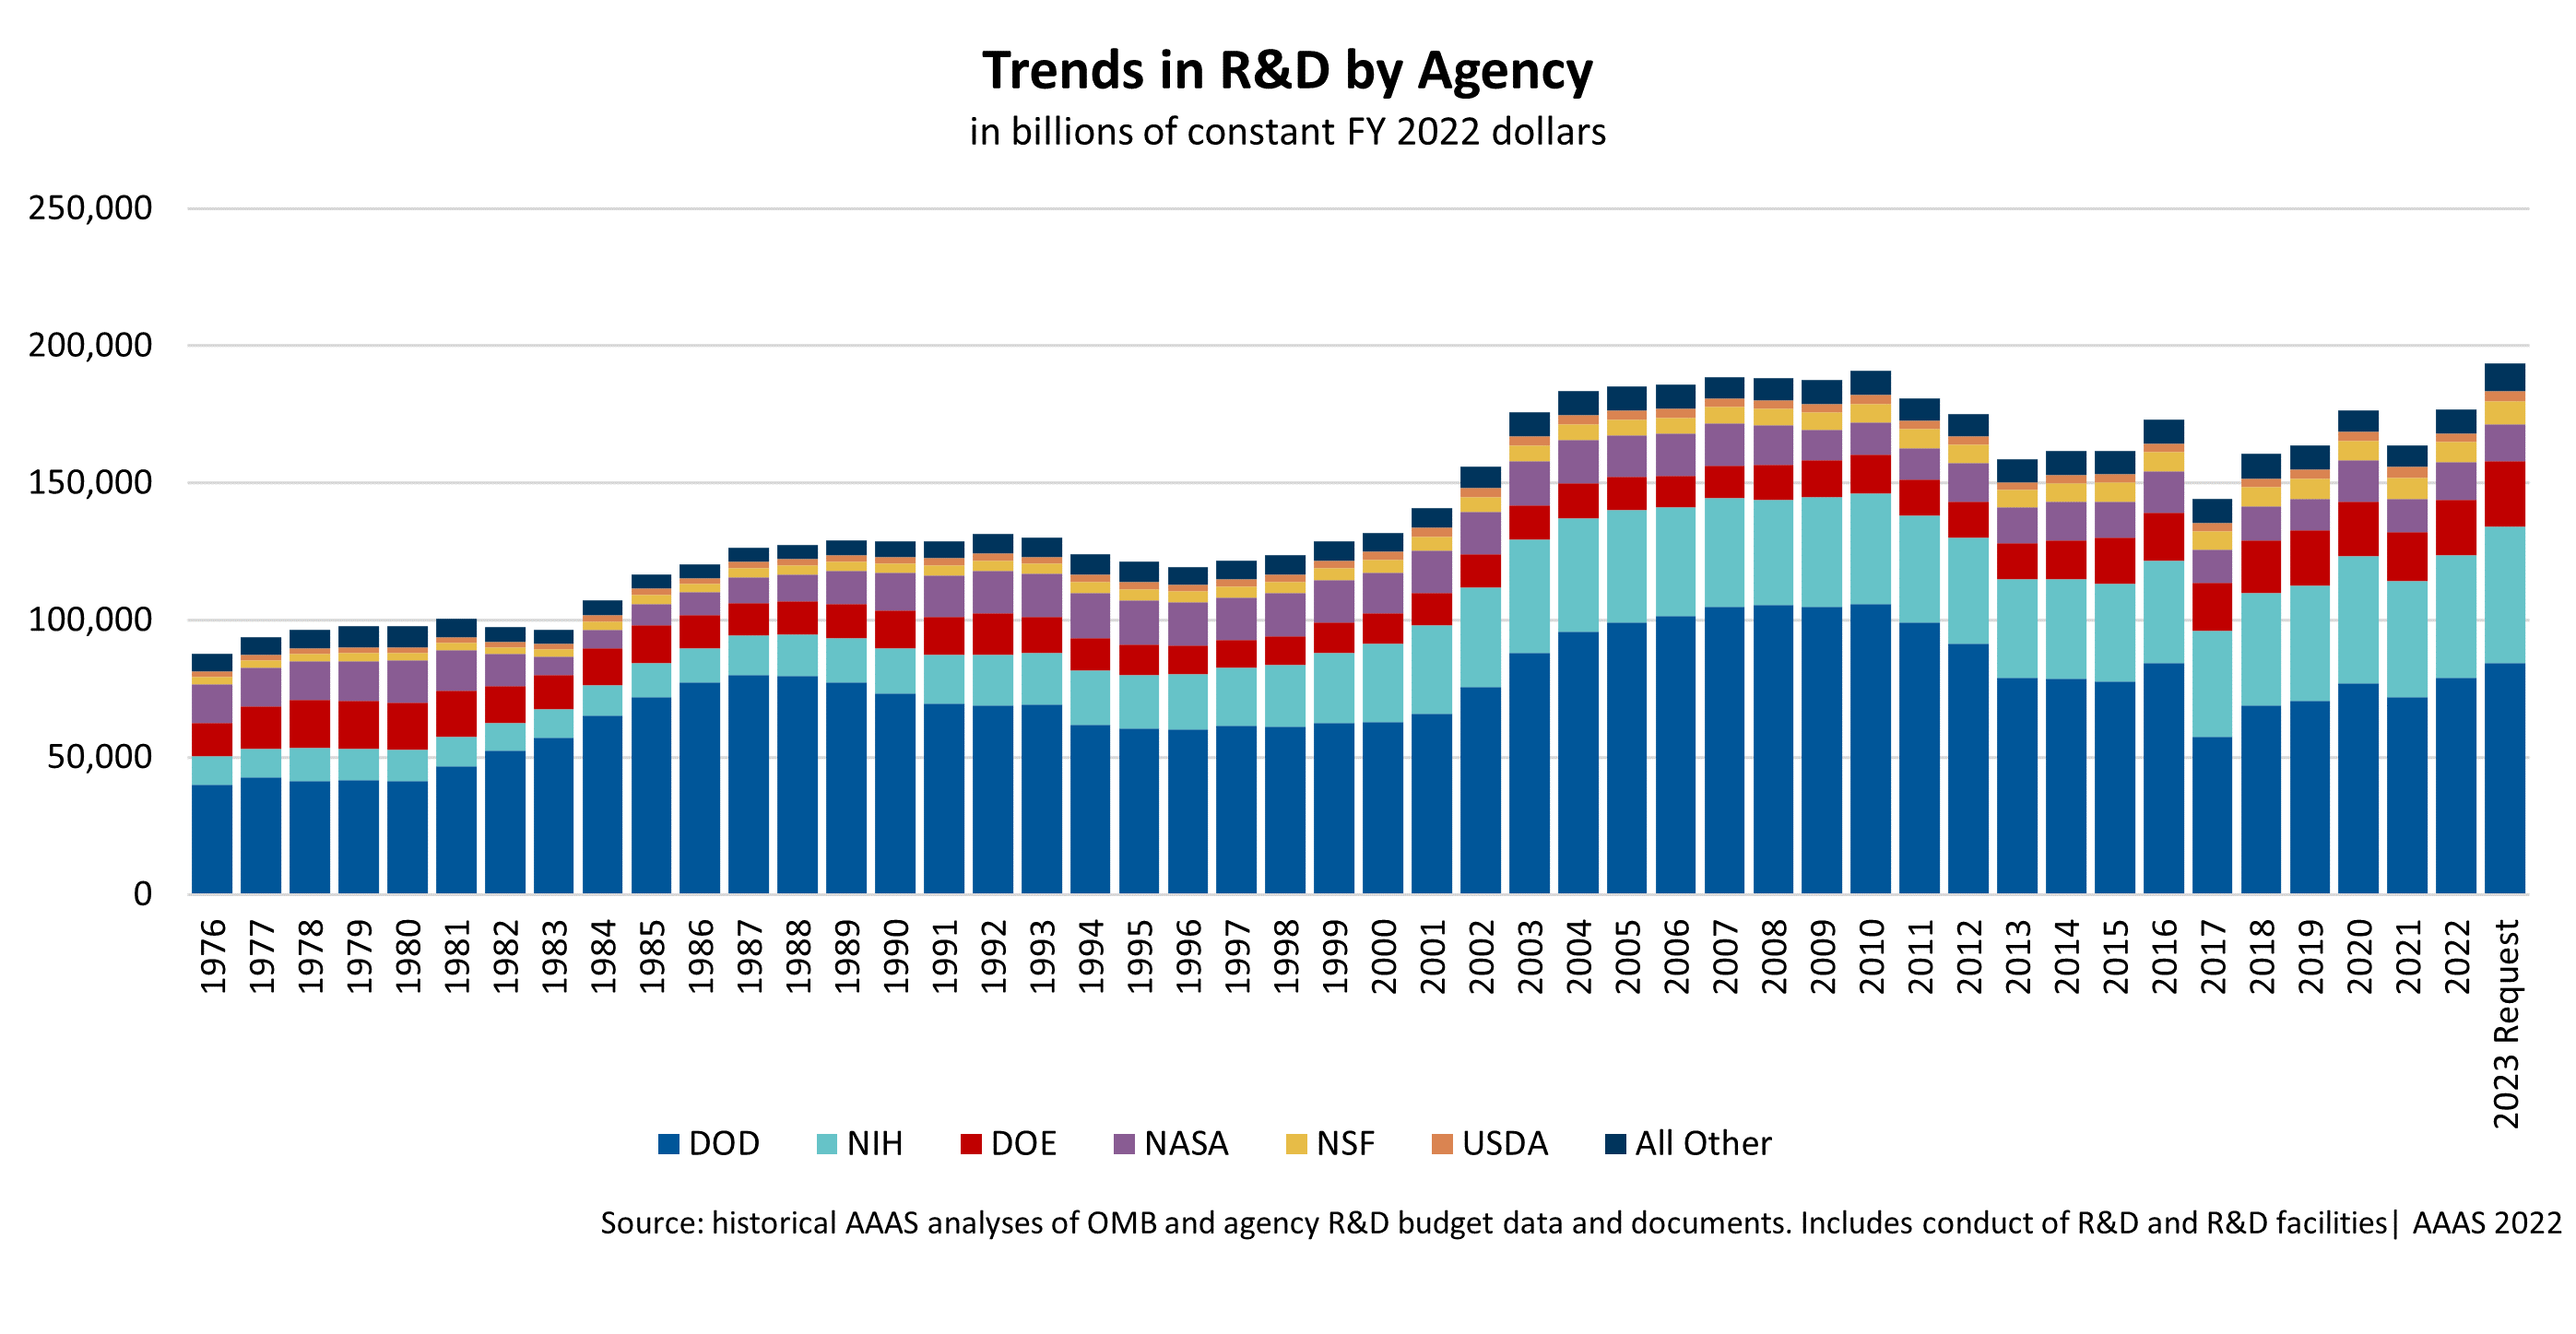
\includegraphics[width=\textwidth]{Agencies.png}
\end{center}
}
\only<2>{
 \begin{center}
 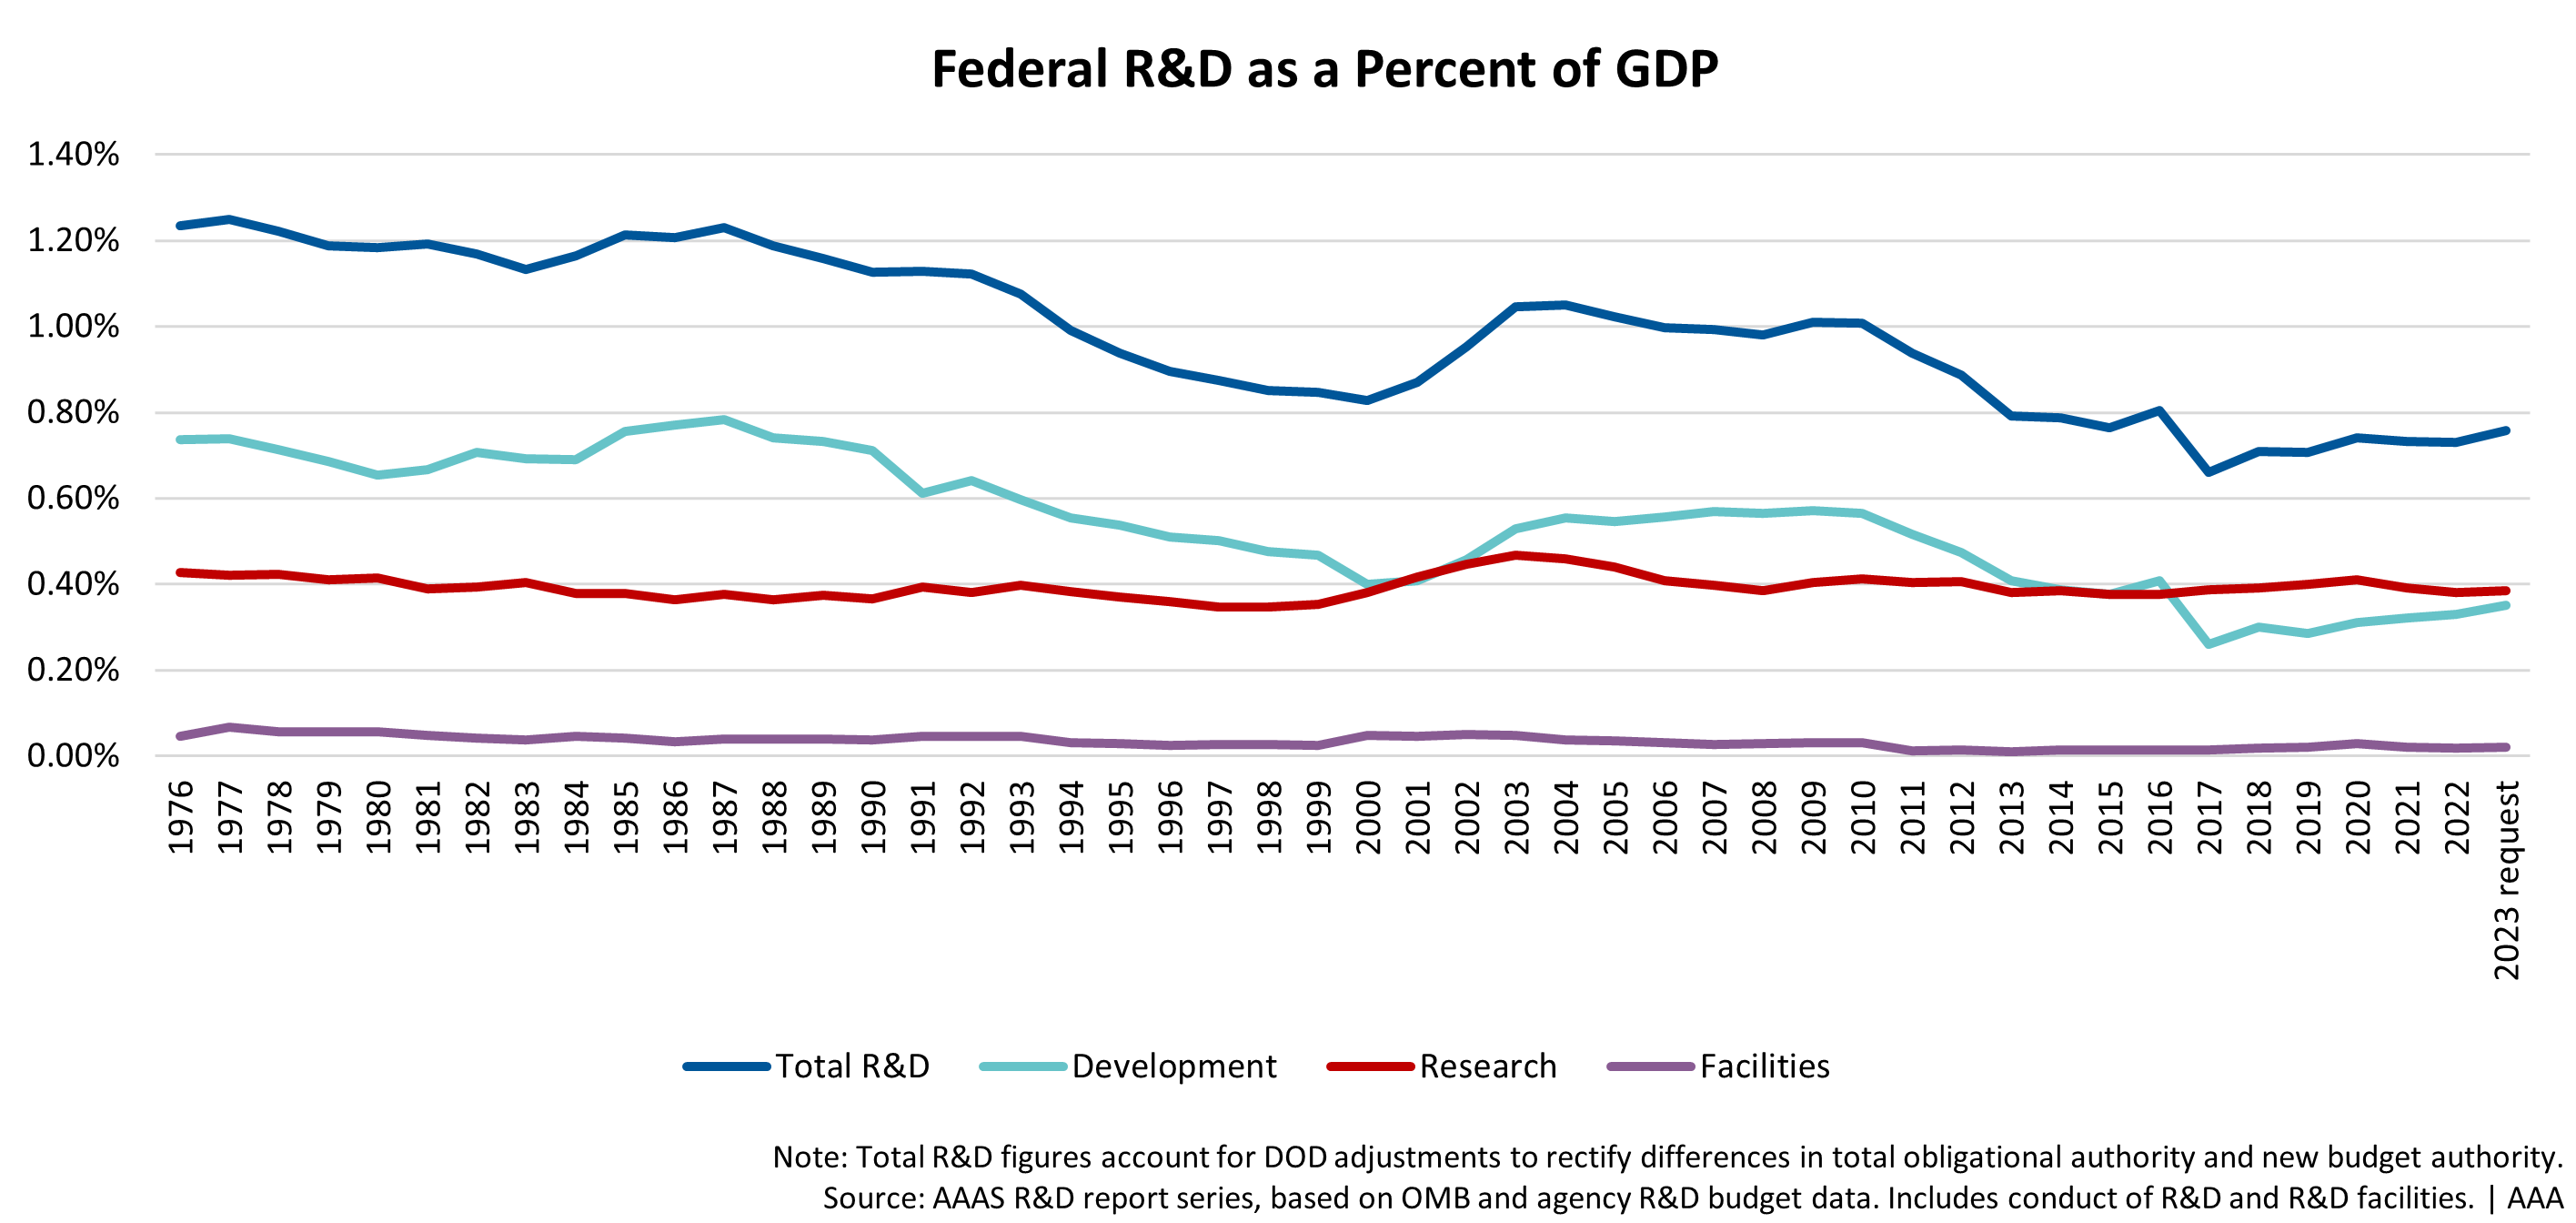
\includegraphics[width=\textwidth]{RDGDP.png}
\end{center}
}
%\only<4>{
% \begin{center}
% 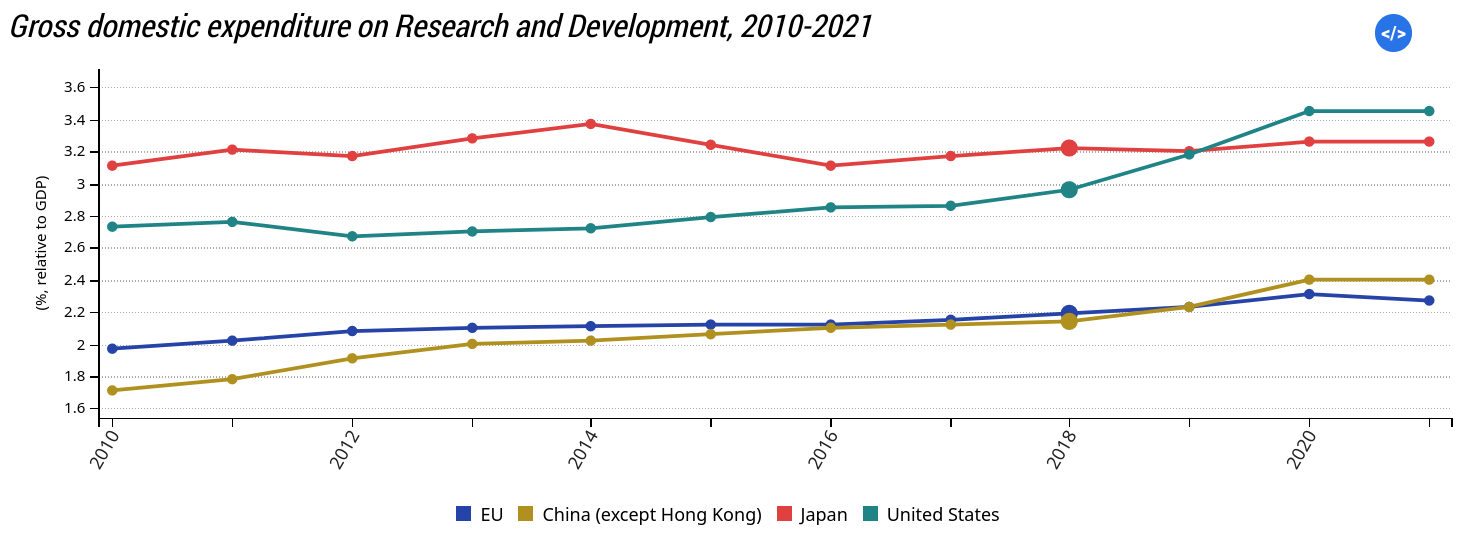
\includegraphics[width=\textwidth]{RDGDP-global.png}
%\end{center}
%}
\end{frame}

 %%%

  \subsection{Symbiotic relation between Publishers and Universities}

 \begin{frame}[t]{New scientific publishing mechanisms}
\begin{itemize}

 \item 1951: Pergamon Press (now \textbf{Elsevier}) and R. Maxwell: many new thematic journals
   %1951: Robert Maxwell creates Pergamon Press. Academic journals used to be mainly owned by learned societies. Maxwell perceives the potential huge profitability of academic publishing as the public funding for research rises. He creates many new journals for specific fields of research and surfs on globalisation with grand titles like ‘International Journal of’. Pergamon Press is sold to Elsevier in 1991. [13]
 \item 1955: appearance of \textbf{impact factor}
   % The idea of an impact factor is first mentioned by Eugene Garfield in Science. It was originally thought of as a tool for librarians to identify journals to purchase, not as a measure of the quality of research [14]. Since 1975, it has been computed and published in the Journal Citation Reports (JCR), nowadays owned by Clarivate [15].
 \item 1970s: rise of journals subscriptions $\Rightarrow$ emerging crisis
   % Beginning of the serials pricing crisis: the prices of subscriptions to scholarly journals rise tremendously. For instance, between 1973 and 1987, the average price increases by 12\% per year, while the costs for the publishers only rise increase by 8\% [16, p. 22]. This difference between expenses and revenue enables the publishers to make big margins. Librarians start to organise and fight back.
 \item 1991: creation free archive \textit{xxx.lanl.gov} at Los Alamos National Laboratory (to become \textbf{arXiv.org}).
% Paul Ginsparg creates the free archive xxx.lanl.gov at Los Alamos National Laboratory, which will become arXiv.org 10 years later [17].
\item By 1994, three years after acquiring Pergamon, Elsevier had raised its prices by 50\%. Librarians began cancelling subscriptions to less popular journals.
\end{itemize}

\fig{.35}{Open_Access_PhD_Comics}
\hspace{1cm}
\fig{.3}{price_increase_publisher_phd_comics}\\
  \begin{center}
    \small
    Graphic from \href{http://www.phdcomics.com/comics.php?f=1533}{PHD Comics}
  \end{center}
\end{frame}

 %%%

 \subsection{Advent of Open Access}

 \begin{frame}[t]{Advent of open access}
\begin{itemize}

\item 2000: Foundation of \textbf{BioMed Central} publisher (now in Springer Nature) and online open-access with \textbf{article processing charge (APC)}
 % Foundation of \textit{BioMed Central} publisher and by Vitek Tracz. This publisher inaugurates a business model based on online open-access journals with an article processing charge (APC). It is now part of Springer Nature. [18]
\item 2000: 34,000 scientists petition:
  \begin{quote}
    “we will publish in, edit and review for, and personally subscribe to only those scholarly and scientific journals that have agreed to grant unrestricted free distribution rights to any and all original research reports.”
  \end{quote}
  Leads to \textbf{the Public Library of Science (PLoS)}, with APC

  \item 2002: \textbf{Budapest Open Access Initiative (BOAI)}: promotes open access \textbf{but} no recommendation for the costs
    %Budapest Open Access Initiative (BOAI). This landmark conference on the open access movement is organised by the Open Society Institute. It results in a public call to promote open access of scholarly literature, insisting on the need to remove all access fees for the readers, but it does not promote any particular model to cover the costs. [20]
  \item 2005: The Wellcome Trust foundation: \textbf{funding requires output open access}
    % The Wellcome Trust, a British research foundation, starts requiring open access for the research they fund. [21]
  \item 2018: \href{https://www.snf.ch/en/bQ17hb9mM1NC4awy/news/news-181010-make-open-access-the-new-normal}{SNF allows to budget OA APC}
  \item 2021: \href{https://www.coalition-s.org/}{The Plan/cOAlition S}: requires Open Access journals or platforms. Followed by \href{https://www.coalition-s.org/supporters/}{many institutions}
    %requires scientific publications resulting from research funded by public grants to be published in compliant Open Access journals or platforms. It is supported by major institutions such as the World Health Organization, the Bill \& Melinda Gates Foundation, the European Commission. [23]
 \end{itemize}
\end{frame}

%%% 


\subsection{Scientific Production so far}
   \begin{frame}[t]{Number of papers produced}

 \begin{quote}
 In 2006, \textbf{50 million} papers have been published since scholarly articles first appeared.\newline Over three centuries, the annual number of published articles has grown exponentially at a \textbf{3\% rate}.
 \end{quote}
 \pause
\begin{minipage}{.6\textwidth}
  \fig{1}{nsb20214-figpbs-001.pdf}\\
  {\tiny \href{https://ncses.nsf.gov/pubs/nsb20214/publication-output-by-country-region-or-economy-and-scientific-field}{National Center for Science and Engineering Statistics}}
\end{minipage}
\pause
 \begin{minipage}{.39\textwidth}
   \fig{.9}{publisher-shares}\\
   {\tiny    \href{https://doi.org/10.5281/zenodo.7212922}{Against Parasite Publishers: Making Journals Free (2022)}}
\end{minipage}
\end{frame}

%%%


\section{Open Access}
\subsection{Open Access models}

\begin{frame}[t]%
 \titleframe{Open Access Models}\vskip1cm%

 
 \begin{itemize}
 \item Gold:
   \begin{itemize}
   \item Immediate open access publication
   \item created by the publisher
   \item made available by publisher online platform
   \item published under a licence that permits reuse (CC) licence.
   \end{itemize}
 \item Green (self-archiving):
   \begin{itemize}
   \item A version of the publication is archived online, e.g., in a repository (arXiv, HAL, infoscience).
   \item does not include the (publisher) work of copyediting, proofreading, typesetting, indexing, metadata tagging, marketing or distribution.
   \item Not listed by publishers (no metrics)
   \item can be freely accessed (with possible embargo period)
   \item Limited licencing
   \end{itemize}

 %\item Bronze
 %  \begin{itemize}
 %  \item free to read and/or download on the publisher’s website
 %  \item closed licence precluding sharing or re-use
 %  \item Authors do not retain the copyright (publisher can withdraw access and the book cannot be shared elsewhere)
 %  \end{itemize}
 %\item Grey
 %  \begin{itemize}
 %  \item Shared online by an academic on personal/social website (researchgate)
 %  \item Illegal if no open licence release nor a Green OA route
 %  \item Tolerated by editors?
 %  \end{itemize}
 %\item Black: Illegal publication

 \end{itemize}
 \vfill
\href{ https://oabooks-toolkit.org/lifecycle/article/13868103-green-gold-diamond-different-models-for-open-access-books}{Credits to oabooks-toolkit}

\end{frame} 
%%%


\subsection{SNF Open Access recommendations}
\begin{frame}[t]{SNF Open access recommendations}

  \begin{center}
    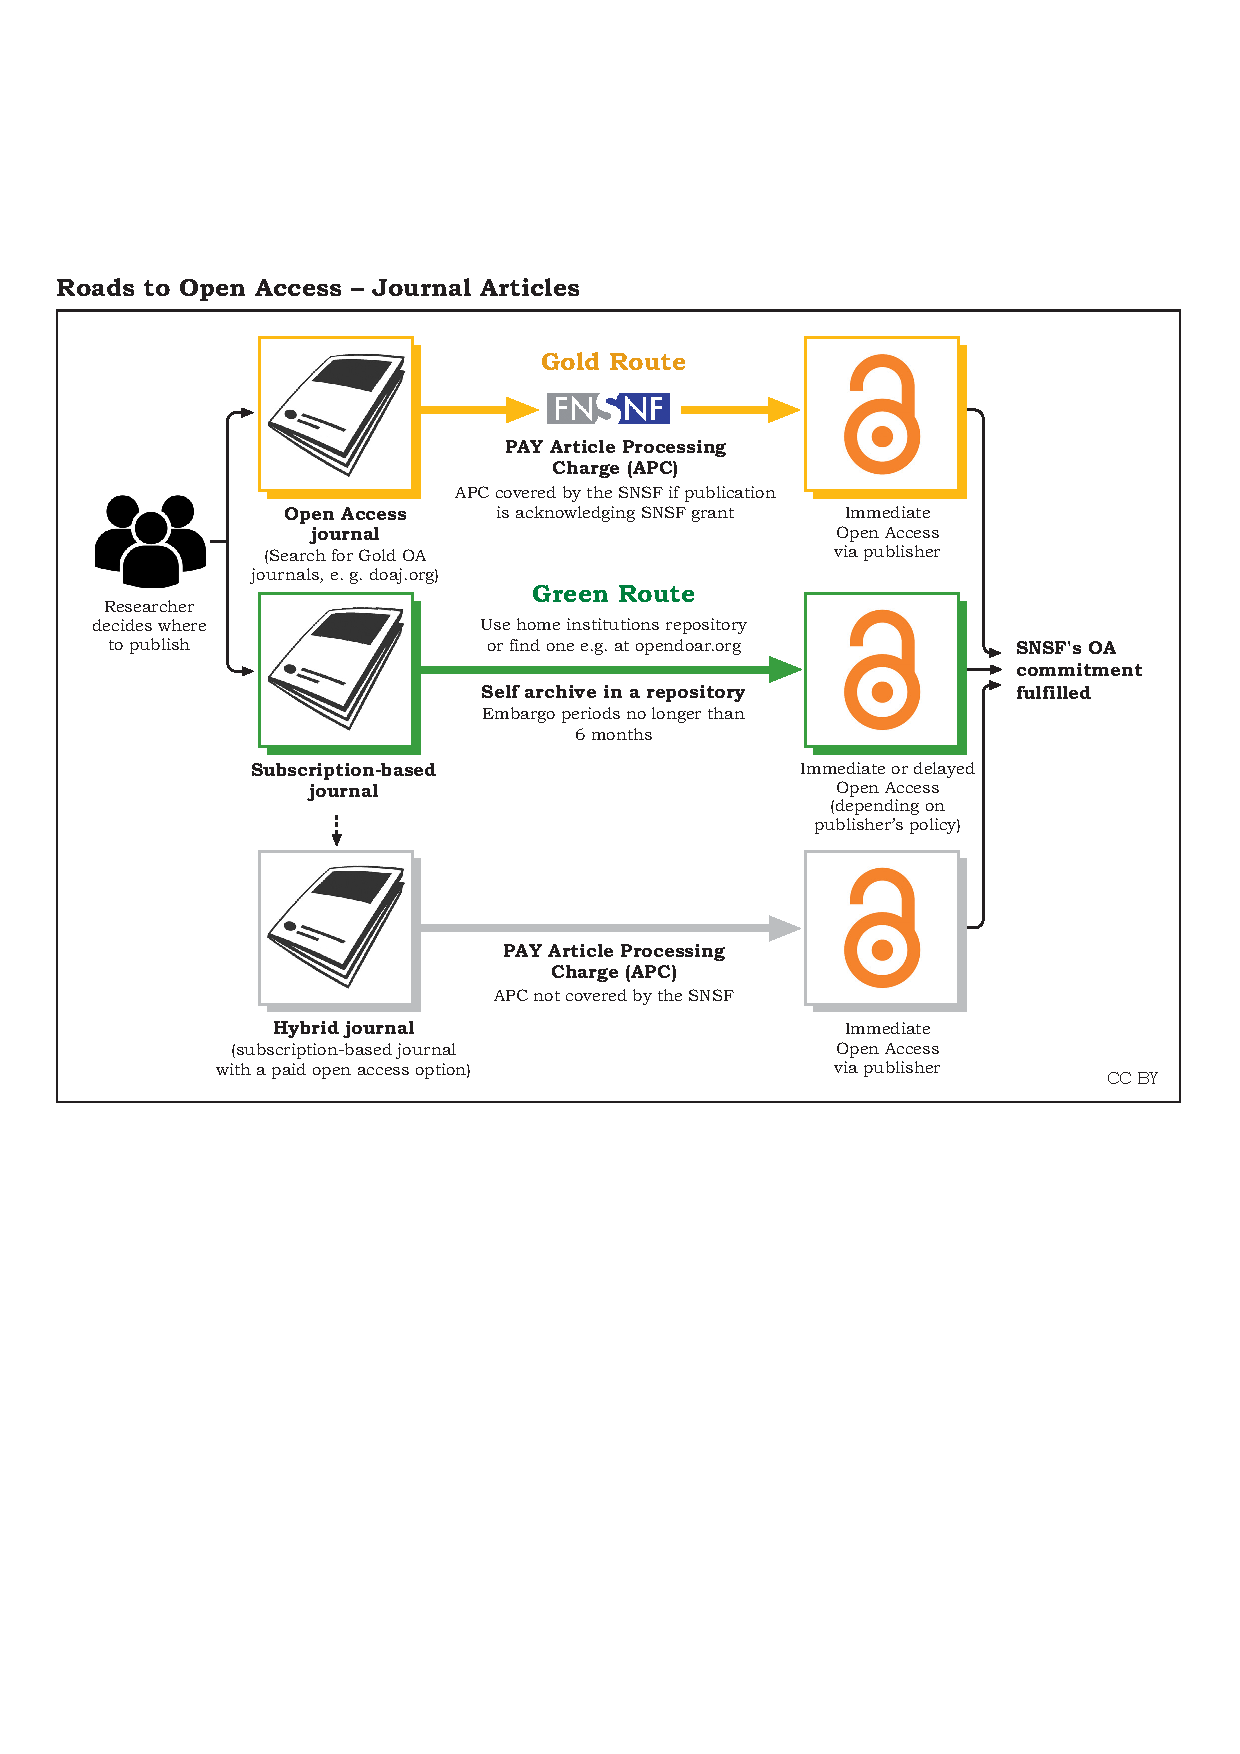
\includegraphics[width=.65\textwidth]{SNSF_Roads_to_OA_Articles}
  \end{center}
  \href{https://www.snf.ch/en/VyUvGzptStOEpUoC/topic/open-access-to-publications}{Illustration from www.snf.ch}
\end{frame}

%%% 

\begin{frame}[t]{What is the problem?}
  \only<1>{\fig{.6}{cash_flow}}
  \only<2>{\fig{.6}{cash_flow_GOA}}
\end{frame}

%%%

\section{Publication Costs}
\subsection{Rigorous publication costs estimation}
\begin{frame}[t]{Cost of a publication?}

\href{https://doi.org/10.12688/f1000research.27468.2}{Grossmann, A. \& Brembs, B. Current market rates for scholarly publishing services. (2021)} 
\begin{quote}
  \vspace{.5cm}
   [...] conservative estimates show that the publication cost for a representative scholarly article \textbf{is around \$400}.
 \end{quote}

 \pause
 \vfill
\centering{
 \Large{How to evaluate such a cost?}}
\end{frame}

%%%

\begin{frame}[t]{Editorial cost of a publication?}
\begin{quote}
  \vspace{-.2cm}
   [...] conservative estimates show that the publication cost for a representative scholarly article \textbf{is around \$400}.
 \end{quote}

  \begin{minipage}{.45\textwidth}
   \textbf{Content acquisition}
   \begin{itemize}
   \item Authors (re-)submission
   \item Dealing with reviewers
   \item Plagiarism/Similarity check
   \item DOI for paper\&reviews
   \item APC collection
   \end{itemize}
 \end{minipage}
 \hfill
   \pause
 \begin{minipage}{.45\textwidth}
   \textbf{Content preparation}
   \begin{itemize}
   \item Manuscript tracking
   \item Production check-in
   \item Manuscript Technical checking
   \item Copyediting, Typesetting, Figures/graphs/tables
   \item Metadata, metrics
   \item Authors corrections
   \end{itemize}
\end{minipage}
\vfill
\pause
\begin{center}
 \begin{minipage}{.7\textwidth}
  \textbf{Dissemination/archiving}
  \begin{itemize}
  \item Web OA platform and hosting
  \item Long-term digital preservation
  \item Distribution to indexing services (Scopus, PMC, DOAJ, ...)
  \end{itemize}
\end{minipage}
\end{center}
%\begin{minipage}{.45\textwidth}
% \end{minipage}
\end{frame}


%%%
\subsection{Article Processing Charges}
\begin{frame}[t]{Cost of APCs?}

  \begin{quote}
   [...] conservative estimates show that the publication cost for a representative scholarly article \alert{is around \$400}.
 \end{quote}
 \pause

 \begin{center}
 \alert{\Large Yet APCs scale with impact factor}\\
 \end{center}

 \pause
 \fig{.6}{publisher-APC}

\end{frame}

%%%

\subsection{Publisher Revenues}
\begin{frame}[t]{Publisher revenues}
 \fig{.5}{publishers-revenues}
 \begin{quote}
   Revenues in 2020 of the biggest publishers in \$

   \href{https://doi.org/10.5281/zenodo.7212922}{Against Parasite Publishers: Making Journals Free (2022)}

 \end{quote}
\end{frame}

%%%
\subsection{Publisher Margins}
\begin{frame}[t]{Publisher margins}
 \fig{.55}{publisher-margins}
 \begin{quote}

   Declared Operating margins in 2020 in \%

   \href{https://doi.org/10.5281/zenodo.7212922}{Against Parasite Publishers: Making Journals Free (2022)}


\end{quote}
\end{frame}

%%%

\section{Diamond Open Access}
\subsection{Definition}

\begin{frame}[t]{Diamond Open Access}

Wikipedia Definition:\newline \newline
 \begin{quote}
   \textbf{Diamond open access} refers to academic texts (such as monographs, edited collections, and journal articles) published/distributed/preserved with \textbf{no fees to either reader or author.} \newline
 \end{quote}
 \pause
\href{https://doi.org/10.5281/zenodo.4558704}{OA Diamond Journals Study. Part 1: Findings. (2021)\newline}

\textbf{Landscape}\\
\begin{itemize}
\item $\sim 29000$ DOA journals (30\% in DOAJ)
\item Fewer articles (356000 per year vs. 453000 APC ones), average $\sim$ 25 articles/year
\item Since 2018 $\searrow$ DOA articles while $\nearrow$ of APC-ones
\item 45\% in Europe, 25\% in Latin America, 16\% in Asia, 5\% in the US/Canada
\item 60\% HSS, 22\% science, 17\% medicine
\end{itemize}

\end{frame}

%%%

\begin{frame}[t]%
 \titleframe{Diamond Open Access}\vskip1cm%

Wikipedia Definition:\newline \newline
 \begin{quote}
   \textbf{Diamond open access} refers to academic texts (such as monographs, edited collections, and journal articles) published/distributed/preserved with \textbf{no fees to either reader or author.} \newline
 \end{quote}

\href{https://doi.org/10.5281/zenodo.4558704}{OA Diamond Journals Study. Part 1: Findings. (2021)\newline}

\textbf{Sustainability and funding}\\
\begin{itemize}
  \item 60\% of DOA journals depend on volunteers
  \item The majority (53\%) run with less than 1 FTE
  \item 70\% declared less than \$/€10,000 annual costs.
  \item Funding mainly by Universities, and much less by Funding agencies
\end{itemize}
\end{frame}

%%%

\subsection{DOA in Switzerland}

\begin{frame}[t]%
 \titleframe{Diamond open in CH}\vskip1cm%


 \href{https://zenodo.org/doi/10.5281/zenodo.7461727}{Mapping the Swiss Landscape of Diamond Open Access Journals. The PLATO Study on Scholar-Led Publishing. Report}\\
 \href{https://www.unige.ch/biblio/fr/actus/projet-plato/}{Projet PLATO: l’Open Access Diamant est en bonne voie en Suisse - Bibliothèque - UNIGE (2023)}

 \begin{minipage}{.49\textwidth}
   \textbf{Key Findings}
   \begin{itemize}
   \item 186 journals
   \item Diverse fields and languages
   \item $< 25$ articles/year
   \item Mostly peer reviewed
   \item Motivation: visibility
   \item SNF policies $\Rightarrow$ DOA move
   \item proofreading well above average
   \item Editorial tasks: (young) volounteers
   \item Sustainability (fundraising) is a challenge
   \item Costs: average CHF 433.03/article (~34 article / year in average)
   \item Open Journal Systems (OJS) platforms
   \end{itemize}
 \end{minipage}
 \begin{minipage}{.49\textwidth}

   \textbf{Key Learnings}
   \begin{itemize}
   \item Driving force: open access best practices
   \item High Quality does not imply equity sacrifice
   \item Should lead to support by funding institutions to
     \begin{itemize}
     \item pay collaborators and improve quality
     \item outsource services (design, hosting, IT development, typesetting)
     \item give recognition to Diamond open access publishing
     \item achieve long-term stability
     \end{itemize}
   \item Funding policies should vary with fields (practices and standards) 
   \item the term \textit{Diamond OA} is intricately linked to a not-for-profit business model based on institutional funding and ownership by the research community, on collaborative work between researchers having shared values of equity and diversity
   \end{itemize}
 \end{minipage}

\end{frame}

%%% 

\subsection{Overlay Journals}

\begin{frame}[t]{Overlay Journals}

 \textbf{Definition}\newline\newline
 \begin{quote}
   An \textbf{open access} academic \textbf{overlay journal} does not produce its own content, but selects from texts that are \textbf{already freely available online}.
 \end{quote}

 
\end{frame}
 
%%%
\begin{frame}[t]

  
\end{frame}
%%%
\begin{frame}[t]
  \fig{.6}{logo2023}
  \begin{itemize}
  \pause
  \item \textbf{Overlay Journal}
   \begin{itemize}
   \item Always a preprint shared on Open Archives (even for refused papers)
   \item Diamond Open Access
   \item FAIR open access (\textbf{F}indable, \textbf{A}ccessible, \textbf{I}nteroperable, \textbf{R}eusable)
   \end{itemize}
   \pause
 \item \textbf{Team}
   \begin{itemize}
   \item Technical board: creators of the journal + data/software editor
   \item Scientific Board: invited
   \item Editorial board: elected
   \item Collegial decisions, no editor in chief
   \end{itemize}
   \pause  
 \item\textbf{Peer Reviewed}
   \begin{itemize}
   \item Publish reviewers' work as Open Reviews
   \end{itemize}
   \pause
 \item\textbf{Data\&Software Review/Curation}
   \begin{itemize}
   \item Strong incentive for \textbf{reproducibility} (ongoing)
   \end{itemize}
   \pause
 \item \textbf{Copy-editing}
   \begin{itemize}
   \item Very high quality
   \item Script to check the correctness of bibliographic entries
   \end{itemize}
 \end{itemize}
\end{frame}


%%%

\section{JTCAM example}
\subsection{Community}

\begin{frame}[t]{JTCAM: Research Community}
\begin{itemize}
 \item Solid Mechanics (Not well aware of Open Access good practices)
 \item Wide spectrum: theoretical, applied, numerical, experimental
 \item Classical journals and publishers
 \begin{itemize}
 \item IJP, JMPS, IJSS, CMAME, IJMM, TI, IJES, Wear, ActaMat (Elsevier)
 \item IJNME, Adv Mat (Wiley)
 \item Comp Mech, Meccanica (Springer)
 \item PRS (Cambridge)
 \item Mechanics of Adv Mat and Struct (Taylor \& Francis)
 \end{itemize}
 \item Alternate journals (Diamond Open Access)
  \begin{itemize}
 \item CRAS (Mersenne)
 \item Archives of Mechanics (since 1950)
 \item Technische Mechanik
 \item Mathematics and Mechanics of Complex Systems (half-diamond)
 \item JACM
 \item ACM
 \end{itemize}
\end{itemize}

\end{frame}

%%%

\begin{frame}[t]{Diamond Open Access Journal in Geomachanics}

  \fig{.4}{ogeo}\\
  {\Large \href{https://opengeomechanics.centre-mersenne.org/}{OpenGeomechanics}}

  \vfill
  \begin{itemize}
  \item WebHost and Funding: Centre Mersenne
  \end{itemize}

  \begin{quote}
    Open Geomechanics is a non-profit, volunteer-run, double blind
 peer-reviewed scientific journal. As a diamond open access journal,
 it is free to publish in and free to read. Open Geomechanics started
 in 2018.\\

 We believe that the time is right to have a journal for geomechanics
 research, edited by geomechanics researchers for geomechanics
 researchers.
\end{quote}
\end{frame}

%%%
\subsection{FAIR principles addressed}
\begin{frame}[t]{JTCAM FAIR principles}
  \textbf{F}indable by Journal indexation
  \begin{itemize}
  \item \textit{Directory of Open Access Journals} (\href{https://doaj.org/}{DOAJ}), \textit{Free Journal Network} (\href{https://freejournals.org/}{FJN}), \textit{International Standard Serial Number International Center} (\href{https://www.issn.org/}{ISSN}), \href{https://reseau-mirabel.info/}{Mir@bel}
  \end{itemize}
\vfill
  \textbf{A}ccessible
  \begin{itemize}
  \item OpenSource \href{https://www.episciences.org/}{Episcience} CMS (funded by French \href{https://www.ccsd.cnrs.fr/}{CCSD} through CNRS, INRIA, INRAE, OpenAIRE, FNSO)  
  \item Overlay Journal: articles stored in open repositories (\href{https://arxiv.org/}{arXiv}, \href{https://hal.science/}{HAL})
  \item Curated/Reviewed Datasets with DOI \href{https://zenodo.org/}{@Zenodo} (\textbf{new})
  \item \href{https://creativecommons.org/share-your-work/cclicenses/}{CC-BY license} 
  \end{itemize}
  \vfill
  \textbf{I}nteroperable
  \begin{itemize}
  \item Provided by the repositories with metadata
  \end{itemize}
\vfill
  \textbf{R}eusable
  \begin{itemize}
  \item Saving Software revision \href{https://www.softwareheritage.org/}{@Software Heritage} (SWHID $\sim$ DOI for software) complement datasets  
  \end{itemize}
 
\end{frame}
 
%%%

\subsection{Publication process}
\begin{frame}[t]{JTCAM: publication process}
 \begin{center}%
   \only<1>{\fig{1}{epirevue_0d}}%
   \only<2>{\fig{1}{epirevue_1d}}%
   \only<3>{\fig{1}{epirevue_2d}}%
    \only<4>{\fig{1}{epirevue_3d}}%
   \only<5>{\fig{1}{epirevue_4d}}%
   \only<6>{\fig{1}{epirevue_5d}}%
 \end{center}%
\end{frame}
 
%%%

\subsection{Data Curation process}
\begin{frame}[t]{Dataset Curation Management}
  \begin{minipage}{.29\textwidth}
    \textbf{Data curation tool}
    \fig{.5}{solidipes}\\
    {\tiny
      \url{https://gitlab.com/dcsm/solidipes}}\newline\newline
    \textbf{funded by\\}
    \fig{.5}{ethr_en_rgb_black}
\end{minipage}
\hfill
\begin{minipage}{.29\textwidth}
  \fig{.5}{logo-renku}
  \fig{.5}{logo-sdsc}
\end{minipage}
\end{frame}

%%%

\subsection{Chronology}
\begin{frame}[t]{JTCAM: Motivation \& Chronology}

 \begin{center}
   \Large
   \textbf{Time to offer an ethical and open publication model}
 \end{center}
\vfill
%\textbf{Historique}
 \begin{itemize}
  \item \parbox{1.5cm}{2015/09} First discussion between V. Acary \& M. Legrand\\[.5em]
  \item \parbox{1.5cm}{2017/07} Online discussion with interested contributors\\[.5em]
  \item \parbox{1.5cm}{2018/05} Steering committee (title, logo, etc)\\[.5em]
  \item \parbox{1.5cm}{2019/06} Scientific committee (25 members)\\[.5em]
  \item \parbox{1.5cm}{2020/01} JTCAM accepted by the Episciences plateform\\[.5em]
  \item \parbox{1.5cm}{2020/05} Editorial committee (10 members)\\[.5em]
  \item \parbox{1.5cm}{2020/08} Official JTCAM kick-off\\[.5em]
  \item \parbox{1.5cm}{2020/09} First submission
  \item \parbox{1.5cm}{2022/10} Referenced in DOAJ
 \end{itemize}

\end{frame}


%%%
\subsection{Costs}
\begin{frame}[t]{JTCAM: costs}
\end{frame}
\subsection{Structural Challenges}

\begin{frame}[t]{JTCAM: Challenges}
  \begin{itemize}
  \item 30 articles published (10 refused)
    \begin{itemize}
    \item Mostly from French community (90\%)
    \item Difficult to become international
    \end{itemize}
  \item Copy-editing
    \begin{itemize}
    \item Low motivation on authors' side
    \item Lots of work for technical editors (about 10h of work per paper)
    \item Fairly long time between acceptation and publication 
    \end{itemize}
  \item Open Data/Open Software 
    \begin{itemize}
    \item Cultural limitations
    \item Development of curation tool (ETH-ORD funding)
    \end{itemize}

  \end{itemize}
\end{frame}

%%%
\subsection{Problematic of science metrics}
\begin{frame}[t]{Community adhesion challenge}

  \textbf{Lack of journal metrics is fearsome for JTCAM authors}
  \begin{itemize}
  \item Authors fear for impact (for young investigators carreers)
  \item Reputation takes time to build
  \item Imbalance between countries incentives (rich vs. poorer countries)
  \end{itemize}

  \vfill
  
  \textbf{San Francisco Declaration on Research Assessment (DORA, 2013)}
  \begin{quote}Do not use journal-based metrics, such as Journal Impact Factors, as a surrogate measure of the quality of individual research articles, to assess an individual scientist’s contributions, or in hiring, promotion, or funding decisions.\end{quote}
   %The declaration is signed by more than 2400 organisations, including universities, funding agencies, and also publishers like Springer-Nature or Elsevier. [22]

\end{frame}
%%%
\begin{frame}[t]{What is the problem?}

\href{https://www.theguardian.com/science/2017/jun/27/profitable-business-scientific-publishing-bad-for-science}{Is the staggeringly profitable business of scientific publishing bad for science?, The Guardian (2017)}

%Scientists are well aware that they seem to be getting a bad deal. The publishing business is “perverse and needless”, the Berkeley biologist Michael Eisen wrote in a 2003 article for the Guardian, declaring that it “should be a public scandal”. Adrian Sutton, a physicist at Imperial College, told me that scientists “are all slaves to publishers. What other industry receives its raw materials from its customers, gets those same customers to carry out the quality control of those materials, and then sells the same materials back to the customers at a vastly inflated price?” (A representative of RELX Group, the official name of Elsevier since 2015, told me that it and other publishers “serve the research community by doing things that they need that they either cannot, or do not do on their own, and charge a fair price for that service”.)

\vfill
\textbf{Researcher}
\begin{quote}
  % Despite my giving sermons all over the world on this topic,
  [...] it seems journals hold sway even more prominently than before. It is that influence, more than the profits that drove the system’s expansion, that most frustrates scientists today
\end{quote}

\textbf{Elsevier}
\begin{quote}
  % Elsevier says its primary goal is to facilitate the work of scientists and other researchers. An Elsevier rep noted that the company received 1.5m article submissions last year, and published 420,000; 14 million scientists entrust Elsevier to publish their results, and 800,000 scientists donate their time to help them with editing and peer-review. “
  We help researchers be more productive and efficient, [...] %” Alicia Wise, senior vice president of global strategic networks, told me. “
  and that’s a win for research institutions, and for research funders like governments
\end{quote}


\textbf{guardian}
\begin{quote}
[...] history shows that betting against science publishers is a risky move. After all, \textbf{back in 1988}, Maxwell predicted that in the future there would only be \textbf{a handful of immensely powerful publishing companies left}, and that they would ply their trade in an electronic age \textbf{with no printing costs}, leading to almost pure profit. 
\end{quote}
\begin{center}
  \textbf{That sounds a lot like the world we live in now}
\end{center}
\end{frame}



%%%

\section{Conclusion}
\begin{frame}[t]{Conclusion}

  \textbf{Where we are}  
  \begin{itemize}
  \item There is value and costs involved in scientific press
    \pause
  \item Gold Open Access releived from the Copyrights issue
    \pause
  \item Yet the APCs are too high
    \pause
  \item Influence of journal metrics remains large (despite of DORA), which locks the market
  \end{itemize}
  \pause
  \vfill
  \textbf{Time for change?}
  \begin{itemize}
  \item If academic press is a market,
    \begin{itemize}
    \item Diamond Open Access can be a concurrent
    \item Breaks monopolies
    \item ``Could'' lower prices
    \item Breaks un-ideal search for sensational
    \end{itemize}
    \pause
  \item Unlike in the past, digitalization and \textit{Open Source} allows Universities to fund infrastructures and services (arXiV, HAL, ...)
    \pause
  \item Saved money can fund repositories (infoscience, research collection, Zenodo), Software development initiatives (ETH-ORD, SNF), or simply research
  \end{itemize}
\end{frame}





\end{document}
